\section{第2讲\quad 空间中的平行关系}
\subsection{夯基础}
\bktopic{点、线确定平面}

\begin{example}[\bkstar{2}{5}]
下列四个条件中，能确定一个平面的条件是
\begin{tasks}(4)
    \task 空间任意三点
    \task 空间两条直线
    \task 空间两条平行直线
    \task 一条直线和一个点
\end{tasks}
\end{example}
\begin{solution}
\textbf{答案：}C

A．当这三个点共线时经过这三点的平面有无数个，故A错

B．当这两条直线是异面直线时，则根据异面直线的定义可得这对异面直线不同在任何一个平面内，故B错

C．根据确定平面的公理的推论可知两条平行直线可唯一确定一个平面，故C对

D．此点在此直线上时有无数个平面经过这条直线和这个点，故D错

故选：C．
\end{solution}

\vspace{2em}

\begin{example}[\bkstar{2}{5}]
空间四点最多可确定平面的个数是
\begin{tasks}(4)
    \task $1$
    \task $2$
    \task $3$
    \task $4$
\end{tasks}
\end{example}
\begin{solution}
\textbf{答案：}D

根据题意知，空间四点确定的直线的位置关系有三种

\ding{172}当空间四点确定的两条直线平行或相交或有且只有三点共线时，则四个点确定 $1$ 个平面

\ding{173}当空间四点确定的两条直线异面时，四点不共面，如三棱锥的顶点和底面上的顶点，则四个点确定 $4$ 个平面

\ding{174}当空间四点在一条直线上时，可确定 $0$ 个平面

故空间四点最多可确定 $4$ 个平面

故选：D．
\end{solution}

\vspace{2em}

\bktopic{直线与平面平行}

\begin{example}[\bkstar{1}{5}]
直线 $l\px\alpha$，在 $\alpha$ 内与 $l$ 平行的直线
\begin{tasks}(4)
    \task 有 $1$ 条
    \task 有 $2$ 条
    \task 有无数条
    \task 不可能有无数条
\end{tasks}
\end{example}
\begin{solution}
\textbf{答案：}C

直线 $l\px\alpha$

则平面 $\alpha$ 内必有一条直线 $m$ 与 $l$ 平行

平面 $\alpha$ 内有无数条直线与 $m$ 平行

则平面 $\alpha$ 内与 $l$ 平行的直线有无数条

故选：C．
\end{solution}

\vspace{2em}

\begin{example}[\bkstar{2}{5}]
在正方体 $ABCD-A_1B_1C_1D_1$ 中，$H$，$E$，$F$，$G$ 分别为 $DC$，$BB_1$，$AA_1$，$CC_1$ 的中点，则与平面 $HFE$ 平行的直线是
\begin{tasks}(4)
    \task $B_1G$
    \task $BD$
    \task $A_1C_1$
    \task $B_1C$
\end{tasks}
\end{example}
\begin{solution}
\textbf{答案：}A

\bkfig{TikZ-final/geometry/solid/p055-o1140.tex}
连接 $B_1G$，$CE$，$FD$

把平面 $HEF$ 延展成平面 $CDFE$

$\because E$，$G$ 分别是 $B_1B$，$C_1C$ 的中点

$\therefore B_1G\px CE$

又 $CE\subset$ 平面 $CDFE$，$B_1G\not\subset$ 平面 $CDFE$

$\therefore B_1G\px$ 平面 $CDFE$

故而 $B_1G\px$ 平面 $HFE$

故选：A．
\end{solution}

\vspace{2em}

\begin{example}[\bkstar{1}{5}]
在正方体 $ABCD-A_1B_1C_1D_1$ 中，$E$ 为 $DD_1$ 的中点，则下列直线中与平面 $ACE$ 平行的是
\begin{tasks}(4)
    \task $BA_1$
    \task $BD_1$
    \task $BC_1$
    \task $BB_1$
\end{tasks}
\end{example}
\begin{solution}
\textbf{答案：}B

\bkfig{TikZ-final/geometry/solid/p055-o1142.tex}
如图，连接 $BD$，与 $AC$ 交于 $O$ 点，则 $O$ 是 $BD$ 中点，连接 $OE$，$BD_1$

又 $\because E$ 为 $DD_1$ 的中点

$\therefore OE\px BD_1$

$\because OE\subset$ 平面 $ACE$，$BD_1\not\subset$ 平面 $ACE$

$\therefore BD_1\px$ 平面 $ACE$

故选：B．
\end{solution}

\vspace{2em}

\begin{example}[\bkstar{1}{5}]
在正方体 $ABCD-A_1B_1C_1D_1$ 中，$M$ 是棱 $CD$ 上的动点，则直线 $MC_1$ 与平面 $AA_1B_1B$ 的位置关系是
\bkfig{TikZ-final/geometry/solid/p012-o0261.tex}
\begin{tasks}(1)
    \task 相交
    \task 平行
    \task 异面
    \task 相交或平行
\end{tasks}
\end{example}
\begin{solution}
\textbf{答案：}B

$\because MC_1\subset$ 平面 $DD_1C_1C$，平面 $AA_1B_1B\px$ 平面 $DD_1C_1C$

$\therefore MC_1\px$ 平面 $AA_1B_1B$

故选：B．
\end{solution}

\vspace{2em}

\begin{example}[\bkstar{2}{5}]
如图，在四棱锥 $P-ABCD$ 中，平面 $PAD\perp$ 平面 $ABCD$，$AB=AD$，$\angle BAD=60^{\circ}$，$E$，$F$ 分别是 $AP$，$AD$ 的中点，求证：直线 $EF\px$ 平面 $PCD$；
\bkfig{TikZ-final/geometry/solid/p012-o0262.tex}
\end{example}
\begin{solution}
在 $\triangle PAD$ 中，因为 $E$，$F$ 分别为 $AP$，$AD$ 的中点

所以 $EF\px PD$

又因为 $EF$ 不在平面 $PCD$ 中，$PD\subset$ 平面 $PCD$

所以直线 $EF\px$ 平面 $PCD$ % 待核对：原书此行末尾多印“PAD”，疑为排版残留，已略去
\end{solution}

\vspace{2em}

\bktopic{平面与平面平行}

\begin{example}[\bkstar{2}{5}]
在正方体 $EFGH-E_1F_1G_1H_1$ 中，平面 $E_1FG_1$ 与平面 $EGH_1$，平面 $FHG_1$ 与平面 $F_1H_1G$，平面 $F_1H_1H$ 与平面 $FHE_1$，平面 $E_1HG_1$ 与平面 $EH_1G$ 中互相平行的对数为
\begin{tasks}(4)
    \task $0$
    \task $1$
    \task $2$
    \task $3$
\end{tasks}
\end{example}
\begin{solution}
\textbf{答案：}B

由图形易得 $E_1F\px H_1G$，$EG\px E_1G_1$，$E_1F\cap E_1G_1=E_1$，$H_1G\cap EG=G$，从而易得平面 $E_1FG_1\px$ 平面 $EGH_1$

在平面 $FHG_1$ 中，$F_1G$ 与 $FG_1$ 相交，则平面 $FHG_1$ 与平面 $F_1H_1G$ 相交

$HH_1\cap FH=H$，则平面 $F_1H_1H$ 与平面 $FHE_1$ 相交

在平面 $EH_1G$ 中，$EH_1$ 与 $E_1H$ 相交，平面 $E_1HG_1$ 与平面 $EH_1G$ 相交

故选：B．
\end{solution}

\vspace{2em}

\begin{example}[\bkstar{2}{5}]
如图所示，在直四棱柱 $ABCD-A_1B_1C_1D_1$ 中，$A_1A=2$，底面是边长为 $1$ 的正方形，$E$，$F$，$G$ 分别是棱 $BB_1$，$AA_1$，$AD$ 的中点，则平面 $A_1DE$ 与平面 $BGF$ 的位置关系是（填“平行”或“相交”）．
\bkfig{TikZ-final/geometry/solid/p013-o0283.tex}
\end{example}
\begin{solution}
\textbf{答案：}平行

\bkfig{TikZ-final/geometry/solid/p056-o1163.tex}
$\because$ 在直四棱柱 $ABCD-A_1B_1C_1D_1$ 中，$A_1A=2$，底面是边长为 $1$ 的正方形

$E$，$F$，$G$ 分别是棱 $BB_1$，$AA_1$，$AD$ 的中点

$\therefore FG\px A_1D$，$A_1F\px BE$

$\therefore$ 四边形 $FBEA_1$ 是平行四边形

$\therefore BF\px A_1E$

$\because BG\cap FG=G$，$A_1D\cap A_1E=A_1$

$BG$，$FG\subset$ 平面 $BGF$，$A_1D$，$A_1E\subset$ 平面 $A_1DE$

$\therefore$ 平面 $A_1DE\px$ 平面 $BGF$

故答案为：平行．
\end{solution}

\vspace{2em}

\begin{example}[\bkstar{2}{5}]
如图，已知四棱锥 $P-ABCD$ 的底面是平行四边形，点 $M$，$N$，$Q$ 分别在 $PA$，$BD$，$PD$ 上，且 $PM:MA=BN:ND=PQ:QD$，求证：平面 $MNQ\px$ 平面 $PBC$．
\bkfig{TikZ-final/geometry/solid/p013-o0284.tex}
\end{example}
\begin{solution}
$\because$ 在 $\triangle PBD$ 中，$BN:ND=PQ:QD$

$\therefore QN\px PB$

又 $QN\not\subset$ 平面 $PBC$，$PB\subset$ 平面 $PBC$

$\therefore QN\px$ 平面 $PBC$

$\because$ 在 $\triangle PAD$ 中，$PM:MA=PQ:QD$

$\therefore MQ\px AD$

又 $AD\px BC$

$\therefore MQ\px BC$

又 $MQ\not\subset$ 平面 $PBC$，$BC\subset$ 平面 $PBC$

$\therefore MQ\px$ 平面 $PBC$

又 $MQ\cap NQ=Q$，$MQ\subset$ 平面 $MNQ$，$NQ\subset$ 平面 $MNQ$

$\therefore$ 平面 $MNQ\px$ 平面 $PBC$
\end{solution}

\vspace{2em}

\subsection{刷中档}
\bktopic{直线与平面平行}

\begin{example}[\bkstar{2}{5}]
下列四个正方体图形中，$A$，$B$ 为正方体的两个顶点，$M$，$N$，$P$ 分别为其所在棱的中点，能得出直线 $AB\px$ 平面 $MNP$ 的图形的序号是
\bkfig[0.6\textwidth]{TikZ-final/geometry/solid/p013-o0286.tex}
\begin{tasks}(4)
    \task \ding{172}\ding{174}
    \task \ding{172}\ding{175}
    \task \ding{173}\ding{174}
    \task \ding{173}\ding{175}
\end{tasks}
\end{example}
\begin{solution}
\textbf{答案：}B

对图\ding{172}，构造 $AB$ 所在的对角面，可以证明这个对角面与平面 $MNP$ 平行，由线面平行的定义可得 $AB\px$ 平面 $MNP$．

对图\ding{175}，通过证明直线 $AB\px PN$ 得到直线 $AB\px$ 平面 $MNP$

对于\ding{173}、\ding{174}无论用定义还是判定定理都无法证明线面平行

故选：B．
\end{solution}

\vspace{2em}

\begin{example}[\bkstar{2}{5}]
如图，在下列四个正方体中，$A$，$B$ 为正方体的两个顶点，$M$，$N$，$Q$ 为所在棱的中点，则在四个正方体中，直线 $AB$ 与平面 $MNQ$ 不平行的是
\begin{tasks}(4)
    \task \raisebox{-.5\height}{\resizebox{0.13\textwidth}{!}{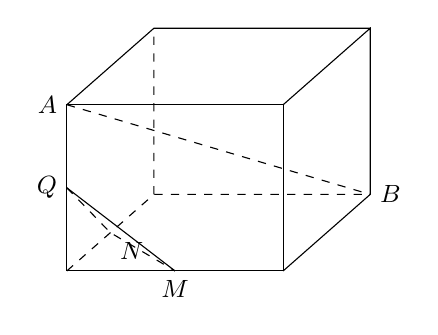
\begin{tikzpicture}[scale=.67, every node/.style={font=\small}]
  \coordinate (FBL) at (0,0);
  \coordinate (FBR) at (4.1,0);
  \coordinate (FTR) at (4.1,3.15);
  \coordinate (FTL) at (0,3.15);
  \coordinate (BBL) at (1.65,1.45);
  \coordinate (BBR) at (5.75,1.45);
  \coordinate (BTR) at (5.75,4.60);
  \coordinate (BTL) at (1.65,4.60);
  \coordinate (M) at (2.05,0);
  \coordinate (Q) at (0,1.575);
  \coordinate (N) at (.825,.725);

  \draw (FBL)--(FBR)--(FTR)--(FTL)--cycle;
  \draw (FTR)--(BTR)--(BBR)--(FBR);
  \draw (FTL)--(BTL)--(BTR);
  \draw[dashed] (FBL)--(BBL)--(BBR) (BBL)--(BTL);
  \draw[dashed] (FTL)--(BBR) (Q)--(N)--(M);
  \draw (Q)--(M);

  \node[left]        at (FTL) {$A$};
  \node[right]       at (BBR) {$B$};
  \node[below]       at (M)   {$M$};
  \node[left]        at (Q)   {$Q$};
  \node[below right] at (N)   {$N$};
\end{tikzpicture}
}}
    \task \raisebox{-.5\height}{\resizebox{0.13\textwidth}{!}{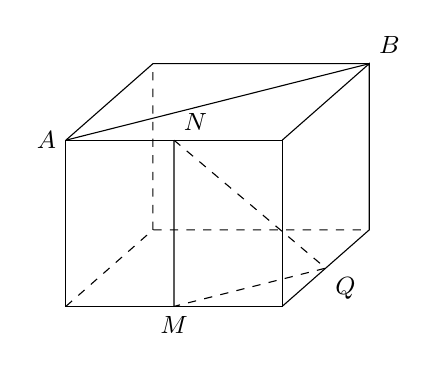
\begin{tikzpicture}[scale=.67, every node/.style={font=\small}]
  \coordinate (FBL) at (0,0);
  \coordinate (FBR) at (4.1,0);
  \coordinate (FTR) at (4.1,3.15);
  \coordinate (FTL) at (0,3.15);
  \coordinate (BBL) at (1.65,1.45);
  \coordinate (BBR) at (5.75,1.45);
  \coordinate (BTR) at (5.75,4.60);
  \coordinate (BTL) at (1.65,4.60);
  \coordinate (M) at (2.05,0);
  \coordinate (N) at (2.05,3.15);
  \coordinate (Q) at (4.925,.725);

  \draw (FBL)--(FBR)--(FTR)--(FTL)--cycle;
  \draw (FTR)--(BTR)--(BBR)--(FBR);
  \draw (FTL)--(BTL)--(BTR);
  \draw[dashed] (FBL)--(BBL)--(BBR) (BBL)--(BTL);
  \draw (FTL)--(BTR) (M)--(N);
  \draw[dashed] (N)--(Q)--(M);

  \node[left]        at (FTL) {$A$};
  \node[above right] at (BTR) {$B$};
  \node[below]       at (M)   {$M$};
  \node[above right] at (N)   {$N$};
  \node[below right] at (Q)   {$Q$};
\end{tikzpicture}
}}
    \task \raisebox{-.5\height}{\resizebox{0.13\textwidth}{!}{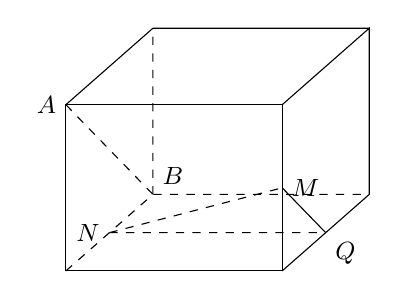
\begin{tikzpicture}[scale=.67, every node/.style={font=\small}]
  \coordinate (FBL) at (0,0);
  \coordinate (FBR) at (4.1,0);
  \coordinate (FTR) at (4.1,3.15);
  \coordinate (FTL) at (0,3.15);
  \coordinate (BBL) at (1.65,1.45);
  \coordinate (BBR) at (5.75,1.45);
  \coordinate (BTR) at (5.75,4.60);
  \coordinate (BTL) at (1.65,4.60);
  \coordinate (M) at (4.1,1.575);
  \coordinate (N) at (.825,.725);
  \coordinate (Q) at (4.925,.725);

  \draw (FBL)--(FBR)--(FTR)--(FTL)--cycle;
  \draw (FTR)--(BTR)--(BBR)--(FBR);
  \draw (FTL)--(BTL)--(BTR);
  \draw[dashed] (FBL)--(BBL)--(BBR) (BBL)--(BTL);
  \draw[dashed] (FTL)--(BBL) (N)--(M) (N)--(Q);
  \draw (M)--(Q);

  \node[left]        at (FTL) {$A$};
  \node[above right] at (BBL) {$B$};
  \node[right]       at (M)   {$M$};
  \node[left]        at (N)   {$N$};
  \node[below right] at (Q)   {$Q$};
\end{tikzpicture}
}}
    \task \raisebox{-.5\height}{\resizebox{0.13\textwidth}{!}{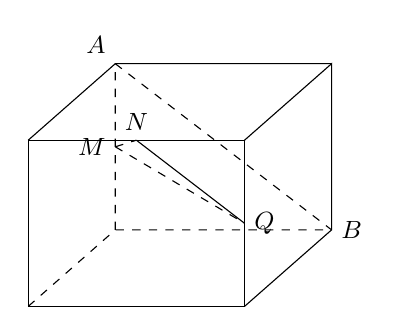
\begin{tikzpicture}[scale=.67, every node/.style={font=\small}]
  \coordinate (FBL) at (0,0);
  \coordinate (FBR) at (4.1,0);
  \coordinate (FTR) at (4.1,3.15);
  \coordinate (FTL) at (0,3.15);
  \coordinate (BBL) at (1.65,1.45);
  \coordinate (BBR) at (5.75,1.45);
  \coordinate (BTR) at (5.75,4.60);
  \coordinate (BTL) at (1.65,4.60);
  \coordinate (M) at (1.65,3.025);
  \coordinate (N) at (2.05,3.15);
  \coordinate (Q) at (4.1,1.575);

  \draw (FBL)--(FBR)--(FTR)--(FTL)--cycle;
  \draw (FTR)--(BTR)--(BBR)--(FBR);
  \draw (FTL)--(BTL)--(BTR);
  \draw[dashed] (FBL)--(BBL)--(BBR) (BBL)--(BTL);
  \draw[dashed] (BTL)--(BBR) (M)--(N) (M)--(Q);
  \draw (N)--(Q);

  \node[above left] at (BTL) {$A$};
  \node[right]      at (BBR) {$B$};
  \node[left]       at (M)   {$M$};
  \node[above]      at (N)   {$N$};
  \node[right]      at (Q)   {$Q$};
\end{tikzpicture}
}}
\end{tasks}
\end{example}
\begin{solution}
\textbf{答案：}A

A．因为直线 $AB$ 与平面 $MNQ$ 相交，所以直线 $AB$ 与平面 $MNQ$ 不平行

B．因为 $AB\px MQ$，且直线 $AB\not\subset$ 平面 $MNQ$，直线 $MQ\subset$ 平面 $MNQ$，所以直线 $AB\px$ 平面 $MNQ$

C．因为 $AB\px MQ$，且直线 $AB\not\subset$ 平面 $MNQ$，直线 $MQ\subset$ 平面 $MNQ$，所以直线 $AB\px$ 平面 $MNQ$

D．因为 $AB\px NQ$，且直线 $AB\not\subset$ 平面 $MNQ$，直线 $NQ\subset$ 平面 $MNQ$，所以直线 $AB\px$ 平面 $MNQ$

故选：A．
\end{solution}

\vspace{2em}

\begin{example}[\bkstar{3}{5}]
如图，在三棱柱 $ABC-A_1B_1C_1$ 中，$AM=2MA_1$，$BN=2NB_1$，过 $MN$ 作一平面交底面三角形 $ABC$ 的边 $BC$，$AC$ 于点 $E$，$F$（$E$、$F$ 与端点不重合），则
\bkfig{TikZ-final/geometry/solid/p014-o0307.tex}
\begin{tasks}(1)
    \task $MF\px NE$
    \task 四边形 $MNEF$ 为梯形
    \task 四边形 $MNEF$ 为平行四边形
    \task $A_1B_1\px NE$
\end{tasks}
\end{example}
\begin{solution}
\textbf{答案：}B

$\because$ 在平行四边形 $AA_1B_1B$ 中，$AM=2MA_1$，$BN=2NB_1$

$\therefore AM\overset{\px}{=}BN$

$\therefore MN\overset{\px}{=}AB$

又 $MN\not\subset$ 平面 $ABC$，$AB\subset$ 平面 $ABC$

$\therefore MN\px$ 平面 $ABC$

又 $MN\subset$ 平面 $MNEF$，平面 $MNEF\cap$ 平面 $ABC=EF$

$\therefore MN\px EF$

$\therefore EF\px AB$，显然在 $\triangle ABC$ 中，$EF\neq AB$

$\therefore EF\neq MN$

所以四边形 $MNEF$ 为梯形

故选：B．
\end{solution}

\vspace{2em}

\begin{example}[\bkstar{2}{5}]
如图，四棱锥 $P-ABCD$ 中，$M$，$N$ 分别为 $AC$，$PC$ 上的点，且 $MN\px$ 平面 $PAD$，则
\bkfig{TikZ-final/geometry/solid/p014-o0309.tex}
\begin{tasks}(1)
    \task $MN\px PD$
    \task $MN\px PA$
    \task $MN\px AD$
    \task 以上均有可能
\end{tasks}
\end{example}
\begin{solution}
\textbf{答案：}B

$\because MN\px$ 平面 $PAD$，$MN\subset$ 平面 $PAC$，平面 $PAC\cap$ 平面 $PAD=PA$，

$\therefore MN\px PA$．

故选：B．
\end{solution}

\vspace{2em}

\begin{example}[\bkstar{3}{5}]
在如图所示的正四棱柱 $ABCD-A_1B_1C_1D_1$ 中，$E$，$F$ 分别是棱 $B_1B$，$AD$ 的中点，直线 $BF$ 与平面 $AD_1E$ 的位置关系是
\bkfig{TikZ-final/geometry/solid/p014-o0311.tex}
\begin{tasks}(1)
    \task 平行
    \task 相交但不垂直
    \task 垂直
    \task 无法确定
\end{tasks}
\end{example}
\begin{solution}
\textbf{答案：}A

取 $AD_1$ 的中点 $O$，连接 $OE$，$OF$，则易得 $OF$ 平行且等于 $BE$
\bkfig{TikZ-final/geometry/solid/p058-o1189.tex}
$\therefore$ 四边形 $BFOE$ 是平行四边形

$\therefore BF\px OE$

$\because BF\not\subset$ 平面 $AD_1E$，$OE\subset$ 平面 $AD_1E$

$\therefore BF\px$ 平面 $AD_1E$

故选：A．
\end{solution}

\vspace{2em}

\begin{example}[\bkstar{3}{5}]
如图，在四棱锥 $P-ABCD$ 中，底面 $ABCD$ 是边长为 $a$ 的正方形，侧面 $PAD\perp$ 底面 $ABCD$，且 $PA=PD=\dfrac{\sqrt{2}}{2}AD$，设 $E$，$F$ 分别为 $PC$，$BD$ 的中点．求证：$EF\px$ 平面 $PAD$．
\bkfig[0.3\textwidth]{TikZ-final/geometry/solid/p015-o0324.tex}
\end{example}
\begin{solution}
\bkfig[0.3\textwidth]{TikZ-final/geometry/solid/p058-o1194.tex}
因为 $ABCD$ 为正方形，连接 $AC$ 交 $BD$ 于点 $F$

又因为在 $\triangle CPA$ 中，$F$ 为 $AC$ 中点，$E$ 为 $PC$ 中点

所以 $EF\px PA$，且 $PA\subset$ 平面 $PAD$，$EF\not\subset$ 平面 $PAD$ % 待核对：原书解析在此处截断，缺少结论句
\end{solution}

\vspace{2em}

\bktopic{平面与平面平行}

\begin{example}[\bkstar{3}{5}]
已知直四棱柱 $ABCD-A_1B_1C_1D_1$，$AD=DD_1=2$，$BC=DC=1$，$DC\perp BC$，$AD\px BC$，$E$，$F$ 分别为 $CC_1$，$DD_1$ 的中点．求证：面 $BEF\px$ 面 $AD_1C_1$．
\bkfig{TikZ-final/geometry/solid/p015-o0325.tex}
\end{example}
\begin{solution}
取 $AD$ 的中点 $G$，连接 $FG$，$BG$，如图所示
\bkfig{TikZ-final/geometry/solid/p059-o1207.tex}
$\because G$ 为 $AD$ 的中点，$AD=2$

$\therefore DG=1$

又 $AD\px BC$，$BC=1$

$\therefore DG\px BC$，$DG=BC$

$\therefore$ 四边形 $BCDG$ 为平行四边形

$\therefore BG\px CD$，$BG=CD$

又 $E$，$F$ 分别为 $CC_1$，$DD_1$ 的中点

$\therefore EF\px CD$，$EF=CD$

$\therefore BG\px EF$，$BG=EF$

$\therefore$ 四边形 $BEFG$ 为平行四边形

$\therefore GF\px BE$

又在 $\triangle ADD_1$ 中，$GF$ 为其中位线

$\therefore GF\px AD_1$

$\therefore AD_1\px BE$

又 $AD_1\not\subset$ 平面 $BEF$，$BE\subset$ 平面 $BEF$

$\therefore AD_1\px$ 平面 $BEF$

由 $E$，$F$ 分别为 $CC_1$，$DD_1$ 的中点，显然有 $C_1D_1\px EF$

又 $C_1D_1\not\subset$ 平面 $BEF$，$EF\subset$ 平面 $BEF$

$\therefore C_1D_1\px$ 平面 $BEF$

$\because AD_1\cap C_1D_1=D_1$

$\therefore$ 面 $BEF\px$ 面 $AD_1C_1$
\end{solution}

\vspace{2em}

\begin{example}[\bkstar{3}{5}]
已知平面 $\alpha\px$ 平面 $\beta$，$P$ 是 $\alpha$，$\beta$ 外一点，过 $P$ 点的两条直线 $PAC$，$PBD$ 分别交 $\alpha$ 于 $A$，$B$，交 $\beta$ 于 $C$，$D$，且 $PA=6$，$AC=9$，$AB=8$，则 $CD$ 的长为
\end{example}
\begin{solution}
\textbf{答案：}$20$ 或 $4$

如图所示，
\bkfig[0.45\textwidth]{TikZ-final/geometry/solid/p059-o1208.tex}
因为平面 $\alpha\px$ 平面 $\beta$

所以 $AB\px CD$

$\therefore \triangle PAB\backsim\triangle PCD$

$\therefore \dfrac{PA}{PC}=\dfrac{AB}{CD}$

$\therefore CD=\dfrac{8\times 15}{6}=20$

当 $P$ 在平面 $\alpha$ 与平面 $\beta$ 之间时

$\therefore \dfrac{PA}{PC}=\dfrac{AB}{CD}$

$\therefore CD=\dfrac{8\times 3}{6}=4$

故答案为：$20$ 或 $4$．
\end{solution}

\vspace{2em}

\bktopic{点共线、线共点问题}

\begin{example}[\bkstar{3}{5}]
如图，三棱锥 $P-ABC$ 中，$M$，$N$ 分别是 $AP$，$AB$ 的中点，$E$，$F$ 分别是 $PC$，$BC$ 上的点且 $\dfrac{PE}{EC}=\dfrac{BF}{FC}=2$，下列命题正确的是
\bkfig{TikZ-final/geometry/solid/p016-o0338.tex}
\begin{tasks}(1)
    \task $MN=EF$
    \task $ME$ 与 $NF$ 是异面直线
    \task $AC\px$ 平面 $MNFE$
    \task 直线 $ME$，$NF$，$AC$ 相交于同一点
\end{tasks}
\end{example}
\begin{solution}
\textbf{答案：}D

依题意，$M$，$N$ 分别是 $AP$，$AB$ 的中点，$E$，$F$ 分别是 $PC$，$BC$ 上的点且 $\dfrac{PE}{EC}=\dfrac{BF}{FC}=2$

所以 $MN\px PB$，$MN=\dfrac{1}{2}PB$，$EF\px PB$，$EF=\dfrac{1}{3}PB$

故A选项错误，B选项错误

易知 $M$，$E\in$ 平面 $APC$，$N$，$F\in$ 平面 $ABC$，平面 $APC\cap$ 平面 $ABC=AC$

设 $ME\cap NF=G$

则由公理 $3$ 知 $G\in AC$

即直线 $ME$，$NF$，$AC$ 相交于同一点 $G$

故D选项正确，C选项错误

故选：D．
\end{solution}

\vspace{2em}

\bktopic{点、线共面}

\begin{example}[\bkstar{2}{5}]
下列四个图形中，正方体棱上的四个中点共面的图形是
\bkfig[0.6\textwidth]{TikZ-final/geometry/solid/p016-o0339.tex}
\begin{tasks}(4)
    \task 甲与乙
    \task 乙与丙
    \task 丙与丁
    \task 丁与甲
\end{tasks}
\end{example}
\begin{solution}
\textbf{答案：}A

分别连接各中点，如图所示
\bkfig[0.6\textwidth]{TikZ-final/geometry/solid/p060-o1221.tex}
观察四个图形，则可发现正方体棱上的四个中点共面的图形是甲与乙

故选：A．
\end{solution}

\vspace{2em}

\subsection{提能力}
\bktopic{点、线确定平面问题}

\begin{example}[\bkstar{3}{5}]
在正方体 $ABCD-A_1B_1C_1D_1$ 中，$E$，$F$ 分别为棱 $AA_1$，$CC_1$ 的中点，则在空间中与三条直线 $A_1D_1$，$EF$，$CD$ 都相交的直线
\begin{tasks}(4)
    \task 不存在
    \task 有且只有两条
    \task 有且只有三条
    \task 有无数条
\end{tasks}
\end{example}
\begin{solution}
\textbf{答案：}D

\bkfig{TikZ-final/geometry/solid/p061-o1234.tex}
在 $EF$ 上任意取一点 $M$

直线 $A_1D_1$ 与 $M$ 确定一个平面

这个平面与 $CD$ 有且仅有 $1$ 个交点 $N$，当 $M$ 取不同的位置就确定不同的平面

从而与 $CD$ 有不同的交点 $N$

而直线 $MN$ 与这 $3$ 条异面直线都有交点．如图

故选：D．
\end{solution}

\vspace{2em}

\begin{example}[\bkstar{3}{5}]
在棱长为 $10$ 的正方体 $ABCD-A_1B_1C_1D_1$ 中，$P$ 为左侧面 $ADD_1A_1$ 上一点，已知点 $P$ 到 $A_1D_1$ 的距离为 $3$，$P$ 到 $AA_1$ 的距离为 $2$，则过点 $P$ 且与 $A_1C$ 平行的直线交正方体于 $P$，$Q$ 两点，则 $Q$ 点所在的平面是
\bkfig{TikZ-final/geometry/solid/p017-o0353.tex}
\begin{tasks}(4)
    \task $ABCD$
    \task $BB_1C_1C$
    \task $CC_1D_1D$
    \task $AA_1B_1B$
\end{tasks}
\end{example}
\begin{solution}
\textbf{答案：}A

如图，设直线 $A_1P$ 与线段 $AD$ 交于点 $E$，连接 $CE$
\bkfig{TikZ-final/geometry/solid/p061-o1236.tex}
可知过点 $P$ 且与 $A_1C$ 平行的直线在平面 $A_1EC$ 内，可知平面 $A_1EC$ 与平面 $ABCD$ 相交于直线 $CE$，点 $Q$ 在直线 $CE$ 上，也在平面 $ABCD$ 内

故选：A．
\end{solution}

\vspace{2em}

\bktopic{直线与平面平行}

\begin{example}[\bkstar{3}{5}]
如图，在各棱长均为 $a$ 的正三棱柱 $ABC-A_1B_1C_1$ 中，$M$，$N$ 分别为线段 $A_1B$，$B_1C$ 上的动点，且 $MN\px$ 平面 $ACC_1A_1$，则这样的 $MN$ 有
\bkfig{TikZ-final/geometry/solid/p017-o0355.tex}
\begin{tasks}(1)
    \task $1$ 条
    \task $2$ 条
    \task $3$ 条
    \task 无数条
\end{tasks}
\end{example}
\begin{solution}
\textbf{答案：}D

由题意得 $A_1B=CB_1=\sqrt{2}a$，在 $BA_1$，$CB_1$ 上分别取 $M$，$N$ 使 $BM=CN$，过 $M$，$N$ 分别作 $MM_1\perp AB$，$NN_1\perp BC$，垂足分别为 $M_1$，$N_1$
\bkfig{TikZ-final/geometry/solid/p061-o1238.tex}
则 $MM_1\px AA_1$，$NN_1\px BB_1$

故 $MM_1\px NN_1$，$\dfrac{BM}{BA_1}=\dfrac{MM_1}{AA_1}$，$\dfrac{CN}{B_1C}=\dfrac{NN_1}{BB_1}$

$\because \dfrac{BM}{BA_1}=\dfrac{CN}{B_1C}$

$\therefore \dfrac{MM_1}{AA_1}=\dfrac{NN_1}{BB_1}$

又 $\because AA_1=BB_1$

$\therefore MM_1=NN_1$，$MM_1\px NN_1$

$\therefore$ 四边形 $MNN_1M_1$ 是平行四边形

$\therefore MN\px M_1N_1$

可得 $M_1N_1\px$ 平面 $ACC_1A_1$

又 $\because MM_1\px$ 平面 $ACC_1A_1$，$M_1N_1\cap MM_1=M_1$

$\therefore$ 平面 $MM_1N_1N\px$ 平面 $ACC_1A_1$，由于 $MN\subset$ 平面 $MM_1N_1N$

所以 $MN\px$ 平面 $ACC_1A_1$，点 $M$，$N$ 是符合 $BM=CN$ 的动点，从而满足条件的 $MN$ 有无数条

故选：D．
\end{solution}

\vspace{2em}

\bktopic{平面与平面平行}

\begin{example}[\bkstar{3}{5}]
如图是正方体的平面展开图，在这个正方体中．
\bkfig[0.35\textwidth]{TikZ-final/geometry/solid/p017-o0356.tex}
\begin{enumerate}
    \item[\ding{172}] $BM\px$ 平面 $DE$
    \item[\ding{173}] $CN\px$ 平面 $AF$
    \item[\ding{174}] 平面 $BDM\px$ 平面 $AFN$
    \item[\ding{175}] 平面 $BDE\px$ 平面 $NCF$
\end{enumerate}
其中正确命题的序号是
\end{example}
\begin{solution}
\textbf{答案：}\ding{172}\ding{173}\ding{174}\ding{175}

把正方体的平面展开图还原成正方体 $ABCD-EFMN$
\bkfig{TikZ-final/geometry/solid/p062-o1252.tex}
\ding{172}$\because BM\px AN$，$BM\not\subset$ 平面 $DE$，$AN\subset$ 平面 $DE$

$\therefore BM\px$ 平面 $DE$，故正确

\ding{173}$\because CN\px BE$，$CN\not\subset$ 平面 $AF$，$BE\subset$ 平面 $AF$

$\therefore CN\px$ 平面 $AF$，故正确

\ding{174}$\because BD\px FN$，$BM\px AN$，$BD\cap BM=B$，$BD$，$BM\subset$ 平面 $BDM$

$FN\cap AN=N$，$FN$，$AN\subset$ 平面 $AFN$

$\therefore$ 平面 $BDM\px$ 平面 $AFN$，故正确

\ding{175}$\because BD\px FN$，$BE\px CN$，$BD\cap BE=B$，$BD$，$BE\subset$ 平面 $BDE$

$FN\cap CN=N$，$FN$，$CN\subset$ 平面 $NCF$

$\therefore$ 平面 $BDE\px$ 平面 $NCF$，故正确

故答案为：\ding{172}\ding{173}\ding{174}\ding{175}．
\end{solution}

\vspace{2em}

\begin{example}[\bkstar{3}{5}]
已知 $E$，$F$，$H$，$G$ 分别是四面体 $ABCD$ 棱 $AB$，$BC$，$CD$，$DA$ 上的点，且 $AE=EB$，$BF=FC$，$CH=2HD$，$AG=2GD$，则下列说法错误的是
\begin{tasks}(2)
    \task $AC\px$ 平面 $EFH$
    \task $BD\px$ 平面 $EFG$
    \task 直线 $EG$，$FH$，$BD$ 相交于同一点
    \task $FE\px GH$
\end{tasks}
\end{example}
\begin{solution}
\textbf{答案：}B

A．$EA=EB$，$BF=FC$，$CH=2HD$，$AG=2GD$，可得到 $GH\px AC$，$EF\px AC$，故得到 $AC\px$ 平面 $EFH$，选项正确

B．因为 $BD$ 和 $FH$ 不平行，而且两条直线在同一平面内，故得到两直线延长后相交，又 $BD\not\subset$ 平面 $EFG$，可得到 $BD$ 与平面 $EFG$ 是相交关系，选项不正确

C．由A选项，结合平行线的传递性得到 $GH\px EF$，则 $EFGH$ 四点共面，且为等腰梯形，延长 $EH$ 和 $FH$ 相交于点 $M$ 则点 $M$ 在 $FH$ 的延长线上，故在平面 $BDC$ 内，同理 $M$ 点也在平面 $ABD$ 内，故 $M$ 应该在两个平面的交线上，即直线 $BD$ 的延长线上，故得证，选项正确

D．$EA=EB$，$BF=FC$，$CH=2HD$，$AG=2GD$，可得到 $GH\px AC$，$EF\px AC$，由平行线的传递性得到 $FE\px GH$，选项正确

故选：B．
\end{solution}

\vspace{2em}

\begin{example}[\bkstar{3}{5}]
如图，在正方体 $ABCD-A_1B_1C_1D_1$ 中，$O$ 为底面 $ABCD$ 的中心，$P$ 是 $DD_1$ 的中点，设 $Q$ 是 $CC_1$ 上的点，当点 $Q$ 在（\quad）位置时，平面 $D_1BQ\px$ 平面 $PAO$．
\bkfig{TikZ-final/geometry/solid/p018-o0369.tex}
\begin{tasks}(1)
    \task $Q$ 与 $C$ 重合
    \task $Q$ 与 $C_1$ 重合
    \task $Q$ 为 $CC_1$ 的三等分点
    \task $Q$ 为 $CC_1$ 的中点
\end{tasks}
\end{example}
\begin{solution}
\textbf{答案：}D

在正方体 $ABCD-A_1B_1C_1D_1$

$\because O$ 为底面 $ABCD$ 的中心，$P$ 是 $DD_1$ 的中点

$\therefore PO\px BD_1$

设 $Q$ 是 $CC_1$ 上的点，当点 $Q$ 在 $CC_1$ 的中点位置时

$PQ\px AB$

$\therefore$ 四边形 $ABQP$ 是平行四边形

$\therefore AP\px BQ$

$\because AP\cap PO=P$，$BQ\cap BD_1=B$，$AP$，$PO\subset$ 平面 $APO$，$BQ$，$BD_1\subset$ 平面 $BQD_1$

$\therefore$ 平面 $D_1BQ\px$ 平面 $PAO$

故选：D．
\end{solution}

\vspace{2em}
